\section{Dense representations from lexicographic optimal chains}

\graphicspath{{images/lexicographic}}

% Intuition
\begin{frame}[t]{Intuition}
	\centering
	\newcommand{\legendsize}{6pt}
	\tikzset{legend/.style = {rectangle, text width=0.2\linewidth}}
	\begin{tikzpicture}
		\onslide<1>{
			\node (pointcloud)
			{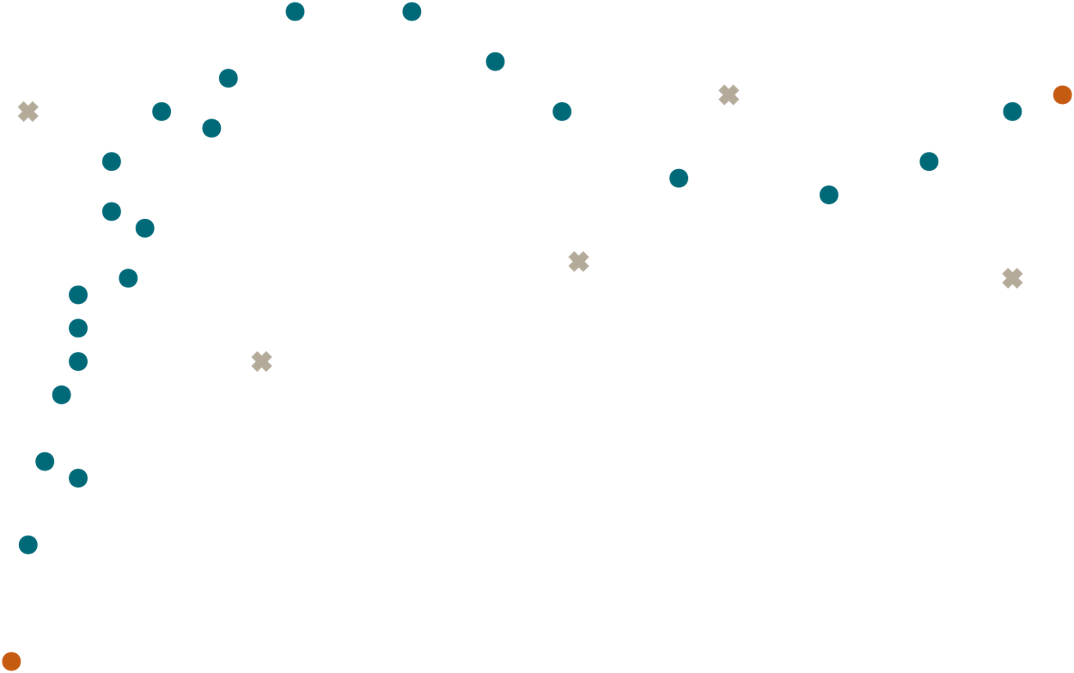
\includegraphics[width=0.8\linewidth]{intuition/state_0}};
		}
		\onslide<2>{
			\node (pointcloud)
			{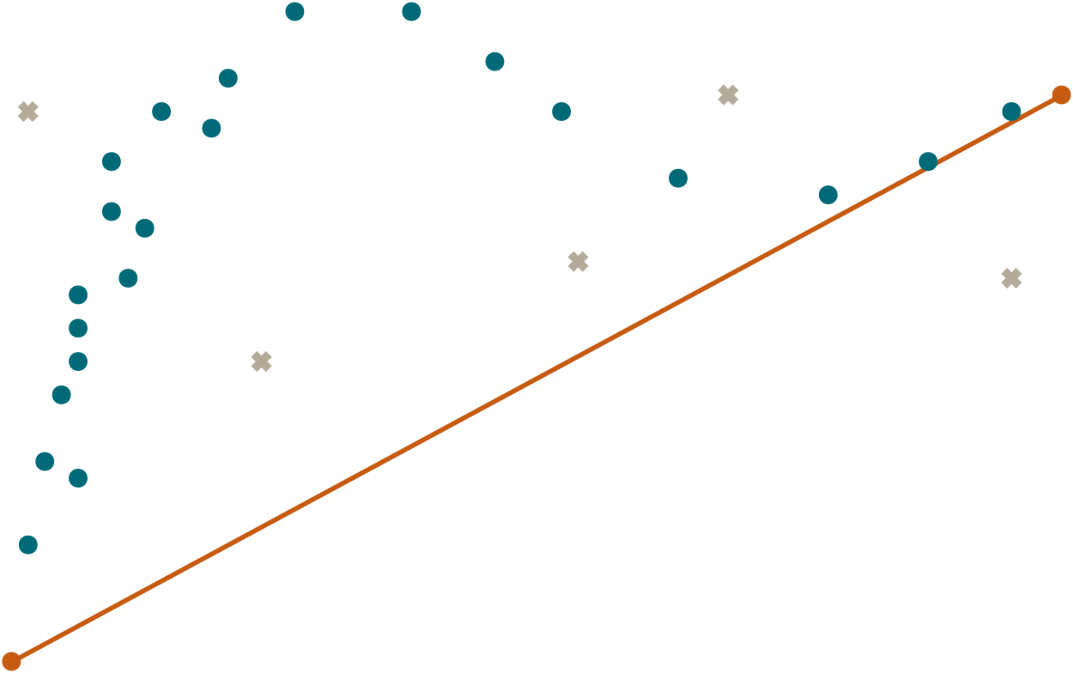
\includegraphics[width=0.8\linewidth]{intuition/state_1}};
		}
		\onslide<3>{
			\node (pointcloud)
			{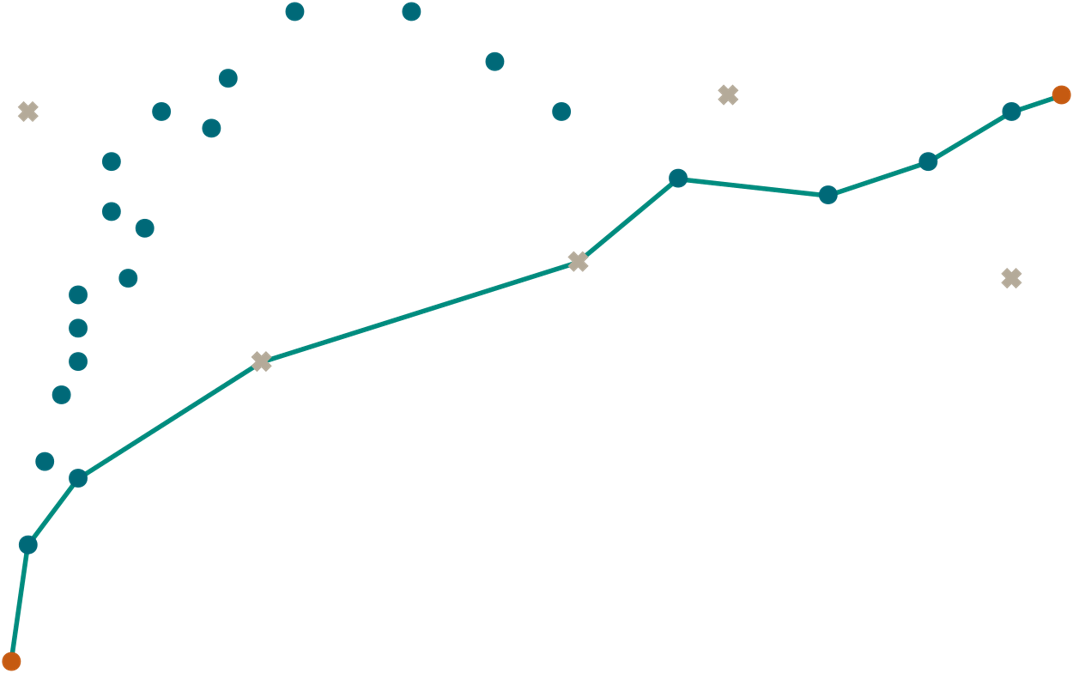
\includegraphics[width=0.8\linewidth]{intuition/state_2}};
		}
		\onslide<4>{
			\node (pointcloud)
			{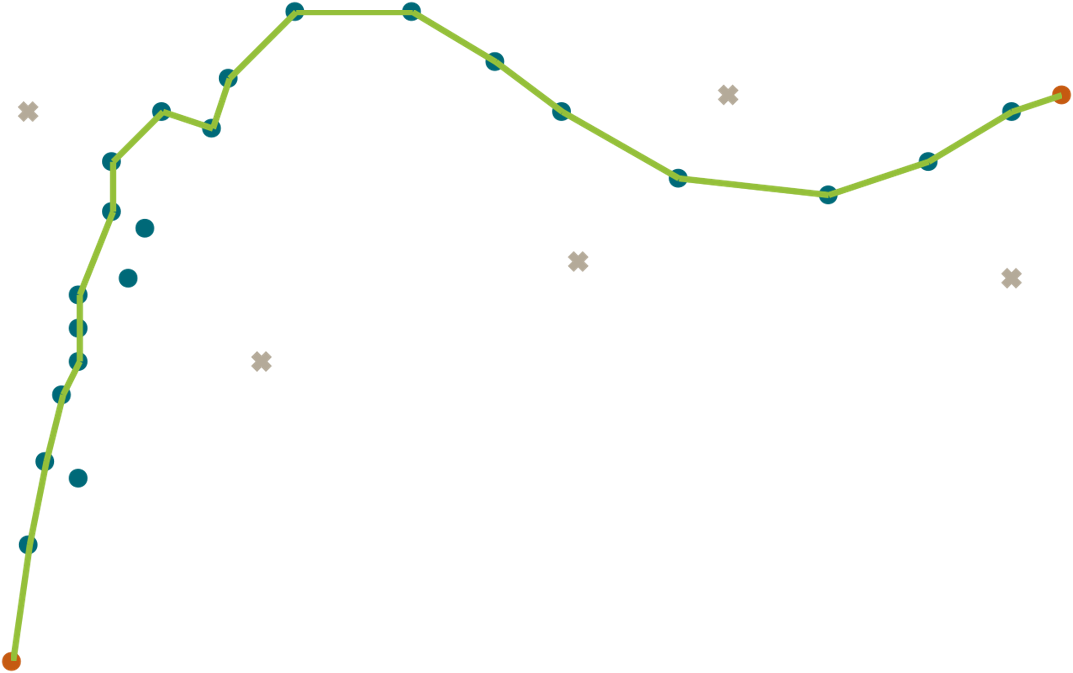
\includegraphics[width=0.8\linewidth]{intuition/state_3}};
		}
		\node[legend, anchor=south east] at (pointcloud.south east){
			\fontsize{\legendsize}{9pt}\selectfont
			\begin{itemize}[itemsep=0pt,partopsep=0pt,topsep=0pt]
				\item[{
\includegraphics[width=\legendsize]{intuition/inlier}}]{Inlier}
				\item[{
\includegraphics[width=\legendsize]{intuition/endpoint}}]{Endpoint}
				\item[{
\includegraphics[width=\legendsize]{intuition/outlier}}]{Outlier}
			\end{itemize}
		};
	\end{tikzpicture}
		
	\begin{center}
		\small
		\only<2>{
		\begin{equation*}
			\min_P \sum_{e \in P} \operatorname{length}(e)
		\end{equation*}
		}
		\only<3>{
		\begin{equation*}
			\min_P \sum_{e \in P} \operatorname{length}(e)^2
		\end{equation*}
		}
		\only<4>{
		\begin{equation*}
			\min_P \sum_{e \in P} \operatorname{length}(e)^p
		\end{equation*}
		}
	\end{center}
\end{frame}

% Crash course
\begin{frame}{Simplicial homology}
	\centering
	\begin{tabular}{ll}
		Simplices & \raisebox{-.5\height}{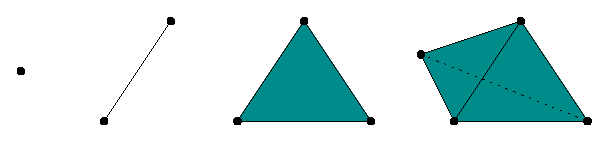
\includegraphics[width=0.5\textwidth]{course/simplices}}
	\end{tabular}
	
	\begin{tabular}{ll} 
		Simplicial complex & \raisebox{-.5\height}{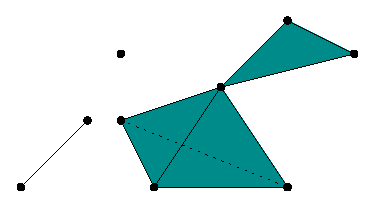
\includegraphics[width=0.4\textwidth]{course/complex}}
	\end{tabular}
	
	A \textbf{\textit{k}-chain} $A$ with coefficients in $\F$ is a formal sum of $k$-simplices:
	\begin{equation*}
		A = \sum_{i} x_i \sigma_i, \text{ with } x_i \in \F \; \text{and} \;\sigma_i \in K^{(k)}
	\end{equation*}
\end{frame}

\begin{frame}{Boundary operator}
	The \textbf{boundary operator} $\partial_k : \Cchains_{k}(K) \to \Cchains_{k-1}(K)$ is the linear map defined for any $k$-simplex $\sigma = [a_0, \dots, a_k]$ as:
	\[
	\partial_k \sigma  \defunder{=}\sum_{i=0}^{k} (-1)^{i} [a_0,\dots, \widehat{a_i},\dots, a_k]
	\]
	
	\begin{center}
		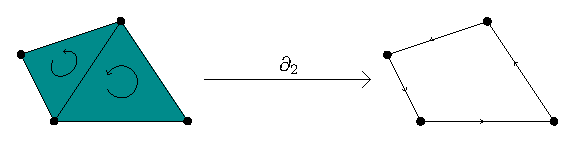
\includegraphics[width=0.8\textwidth]{course/boundary}
	\end{center}
\end{frame}

\begin{frame}{Cycles \& Boundaries}
	The kernels and images of the boundary operator form respectively the vector space of \textbf{cycles} and \textbf{boundaries}:
	\begin{align*}
		\Zchains_{k}(K) &\defunder{=} \Ker \partial_k = \Big\{ \Gamma \in \Cchains_{k}(K), \partial_k \Gamma = 0 \Big\} 
		%\label{definition:absolute-cycles}
		\\
		\Bchains_k(K) &\defunder{=} \Ima \partial_{k+1} = \Big\{ \Gamma \in \Cchains_{k}(K), \exists A \in \Cchains_{k+1}(K) \mid \Gamma = \partial_{k+1} A \Big\} 
		%\label{definition:absolute-boundaries}
	\end{align*}
\end{frame}

\begin{frame}{Boundaries have no boundaries}
	Fundamental property
	\begin{tabular}{ll}
	$\partial_{k} \partial_{k+1} = 0$ & "Boundaries have no boundaries" \\
	\pause
	$\Bchains_k(K) \subset \Zchains_k(K)$ & "All boundaries are cycles"
	\end{tabular}

	\pause
	\begin{center}
		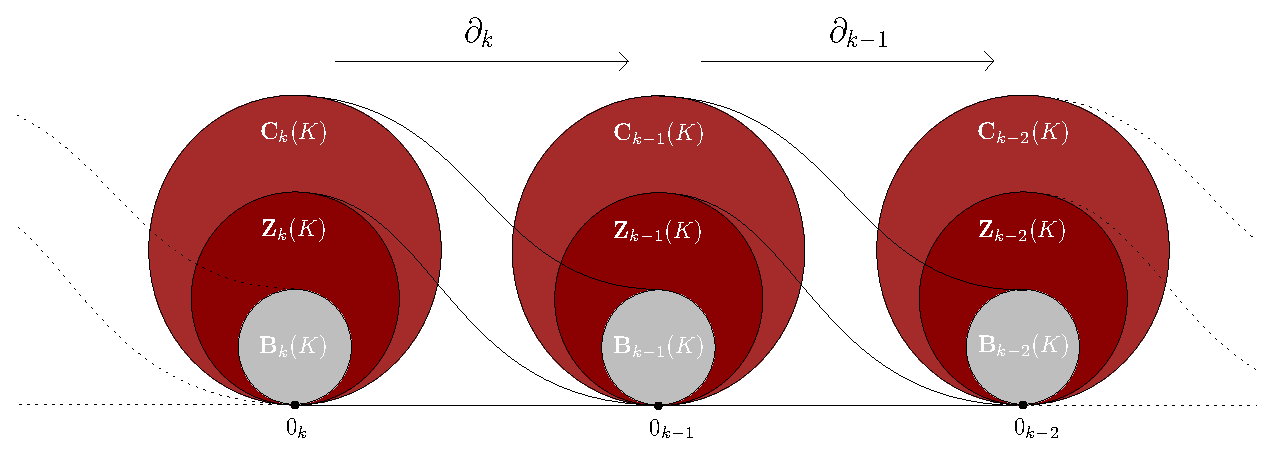
\includegraphics[width=\textwidth]{course/sequence}
	\end{center}
\end{frame}


% Codimension 1: Algorithm
\begin{frame}
	\begin{minipage}[t][0.5\textheight][t]{0.8\linewidth}
		\scriptsize
		\begin{algorithm}[H]
			%			\caption{Lexicographic min-cut}\label{algorithm:Lex-OHCP}
			\SetKwInOut{Input}{Inputs}
			\SetKwInOut{Output}{Output}
			\SetKw{Continue}{continue}
			\SetKw{Or}{or}
			\Input{$G = (\GraphV, \GraphE)$ and $\alpha_1, \alpha_2 \in \GraphV$, with $\GraphE=\{e_i,i=1,\dots,n\}$ in decreasing order}
			\Output{$\Gamma_{\operatorname{LMC}}$}
			\alert<+>{$\Gamma_{\operatorname{LMC}} \leftarrow \varnothing$} \\
			\alert<+>{\For{$v \in \GraphV$} {
					\textbf{MakeSet}(v)
			}}
			
			\For{$e \in \GraphE$ in decreasing order}{
				\alert<+>{$e = (v_1, v_2) \in \GraphV\times \GraphV$} \\
				\alert<+>{$r_1 \leftarrow \textbf{FindSet}(v_1)$, $r_2 \leftarrow \textbf{FindSet}(v_2)$ \\
					$c_1 \leftarrow \textbf{FindSet}(\alpha_1)$, $c_2 \leftarrow \textbf{FindSet}(\alpha_2)$} \\
				\eIf{\alert<+>{$\{ r_1, r_2\} = \{ c_1, c_2 \}$}}{
					$\Gamma_{\operatorname{LMC}} \leftarrow \Gamma_{\operatorname{LMC}} \cup e$
				}
				{
					$\textbf{UnionSet}(r_1, r_2)$
				}
			}
		\end{algorithm}
	\end{minipage}		
\end{frame}